\chapter{Introduction}
\label{ch:intro}

About the definition

\begin{definition}


% Here is a comment.
section/def section/def section/def
section/def section/def
\end{definition}


About thenext definition.
text that will be dropped we can also put latex  \textbf{Zero}.
here is some $math$
% I can alno put comments here

\begin{definition}[Definition \textbf{Zero}]
% Here is a comment.
section/def section/def section/def
section/def section/def
\end{definition}

This is a postamble.

\section{Roadmap}
\label{sec:roadmap}



\begin{definition}[Definition \textbf{One}]
\label{def:one}
section/def section/def section/def
section/def section/def
\end{definition}



\subsection{Roadmap subsection}

\subsubsection{Roadmap subsubsection}
\paragraph{This is a paragraph inside a subsubsection}

\begin{group}[Group title 0]
\begin{definition}[Definition $\mathrm{Title}$]
\label{def:title}
  def def def
  def
  def def.
\end{definition}
\end{group}


This is the preamble to this group.
\begin{group}[Group Title]
  
\begin{definition}[Definition $\mathrm{Title}$]
\label{def:title}
  def def def
  def
  def def.
\end{definition}



\begin{example}[Example \textbf{Title}]
\label{ex:title}
  ex ex ex
  ex
  ex ex.
  \begin{center}
  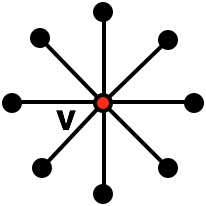
\includegraphics[width=1.5in]{./media-star/star-graph1.jpg}
  \end{center}
\end{example}
\end{group}

Here is some postamble text.
ALso $\mathbf{math}$
%% ALso comments.
Hope it works.
